
\TODO

\begin{itemize}
    \item example dma written in verilog, driver nonfunctional for linux > 2.26 (approx)
    \item chose native linux driver, files under /sys/devices/pci
\end{itemize}

\todo{overview}

\begin{figure}[!ht]
    \centering
    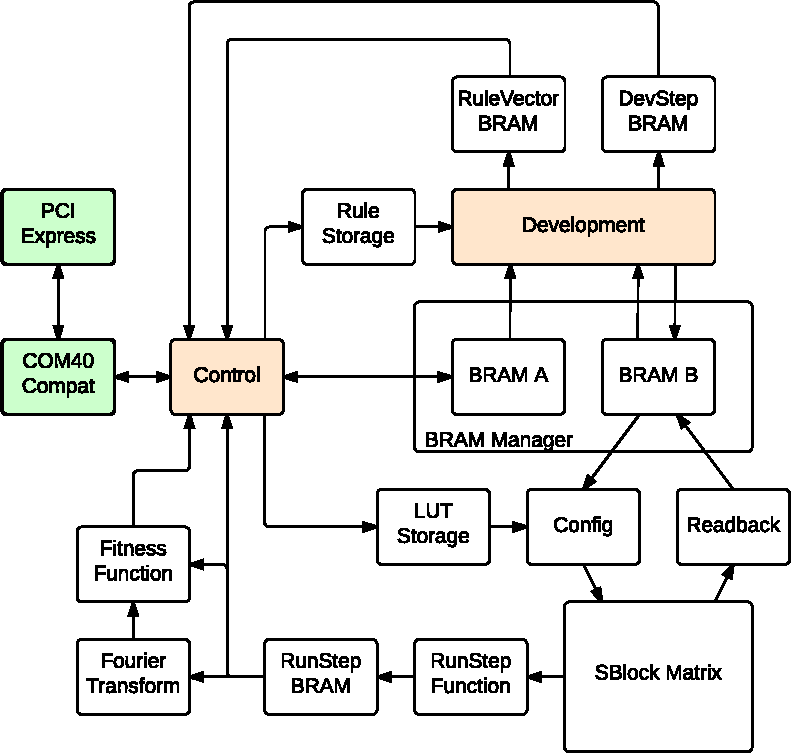
\includegraphics[width=0.48\textwidth]{figures/overview-lundal}
    \caption{Lundal's additions in green}
    \label{fig:overview-lundal}
\end{figure}

\todo{describe com module}

\begin{figure}[!ht]
    \centering
    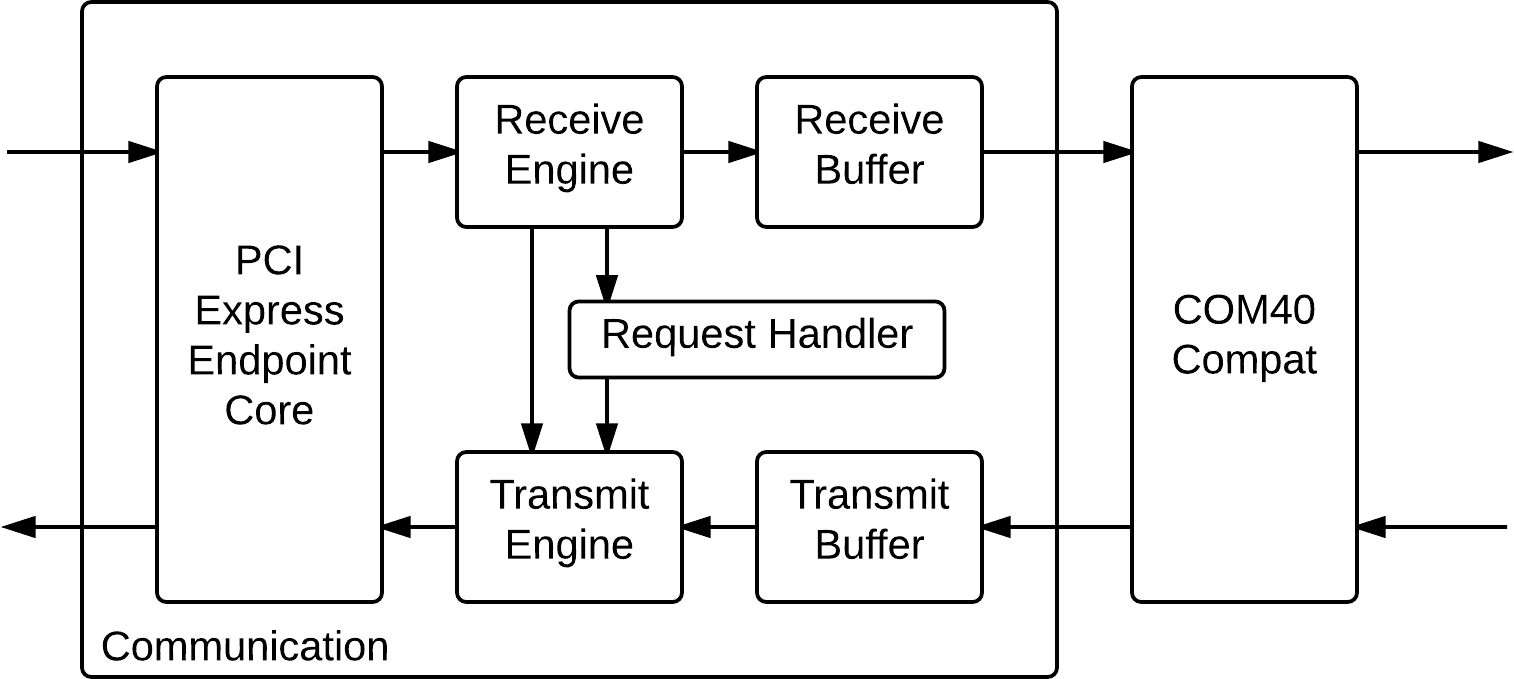
\includegraphics[width=0.48\textwidth]{figures/details-communication}
    \caption{Detailed block-diagram of the PCI Express communication module.}
    \label{fig:details-communication}
\end{figure}

\todo{describe reception engine}

\begin{figure}[!ht]
    \centering
    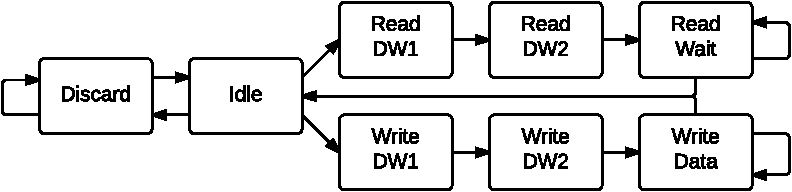
\includegraphics[width=0.48\textwidth]{figures/statemachine-receive}
    \caption{State machine of the reception engine.}
    \label{fig:statemachine-receive}
\end{figure}


\todo{describe transmission engine}

\begin{figure}[!ht]
    \centering
    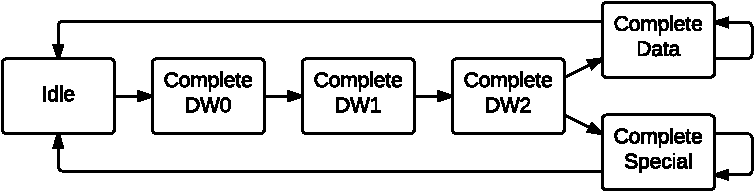
\includegraphics[width=0.48\textwidth]{figures/statemachine-transmit}
    \caption{State machine of the transmission engine.}
    \label{fig:statemachine-transmit}
\end{figure}

\todo{describe fifo buffers}

\begin{figure}[!ht]
    \centering
    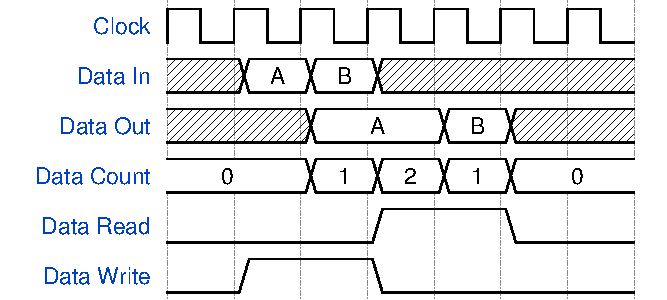
\includegraphics[width=0.40\textwidth]{figures/wavediagram-fifo}
    \caption{Wave diagram for a FIFO buffer. It shows two consecutive writes followed by two consecutive reads.}
    \label{fig:wavediagram-fifo}
\end{figure}

Notice how the read signal needs to be asserted before the clock tick when data is read to ensure correct consecutive reads.
This is due to the BRAM used within the FIFO, which updates at the clock tick.
Therefore, the address has to be updated before the clock tick (by the read signal) to have correct data available for a read in the following cycle.

